

\textit{Special Function Units (SFUs)} are a approximation units, which computes fast approximations of transcendental functions such as sine, cosine, reciprocal and square root.
%Each SFU also features four floating-point multipliers that can offer extra FP throughput in addition to SPs. The SFU pipelines are independent from the SP pipelines. 
% GPU Performance Modeling and Optimization cpt 6
% Add cite

\begin{figure}[H]
	\centering
	\fbox{
		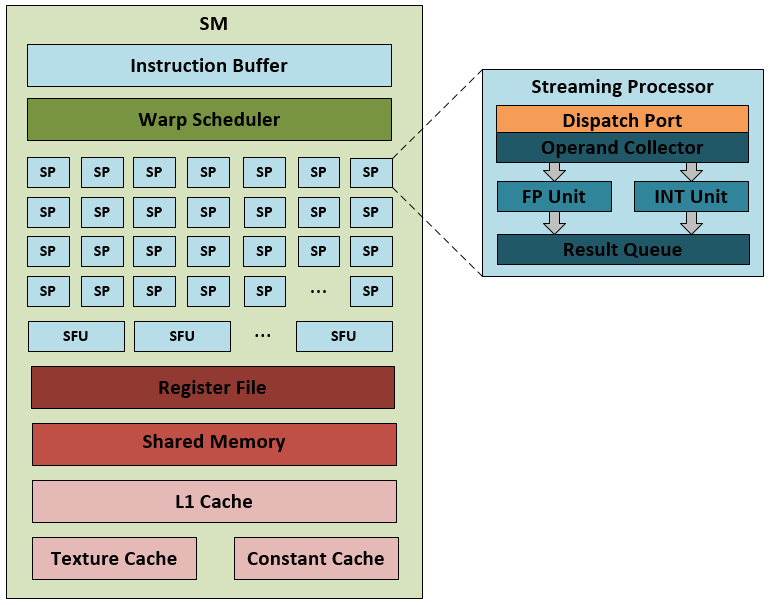
\includegraphics[width=1\textwidth]{figs/hw/hw-sm} }
	\caption{TBD}
	\label{fig:hw-sm}
\end{figure}